% -*- TeX-engine: xetex; eval: (auto-fill-mode 0); eval: (visual-line-mode 1); -*-
% Compile with XeLaTeX

%%%%%%%%%%%%%%%%%%%%%%%
% Option 1: Slides: (comment for handouts)   %
%%%%%%%%%%%%%%%%%%%%%%%

\documentclass[slidestop,compress,mathserif,12pt,t,professionalfonts,xcolor=table]{beamer}

% solution stuff
\newcommand{\solnMult}[1]{
\only<1>{#1}
\only<2->{\red{\textbf{#1}}}
}
\newcommand{\soln}[1]{\textit{#1}}

%%%%%%%%%%%%%%%%%%%%%%%%%%%%%%%
% Option 2: Handouts, without solutions (post before class)    %
%%%%%%%%%%%%%%%%%%%%%%%%%%%%%%%

% \documentclass[11pt,containsverbatim,handout,xcolor=xelatex,dvipsnames,table]{beamer}

% % handout layout
% \usepackage{pgfpages}
% \pgfpagesuselayout{4 on 1}[letterpaper,landscape,border shrink=5mm]

% % solution stuff
% \newcommand{\solnMult}[1]{#1}
% \newcommand{\soln}[1]{}

% % % This breaks things for me for some reason.
% % tell pgfpages how to set page sizes in XeLaTeX
% %\renewcommand\pgfsetupphysicalpagesizes{%
% %   \pdfpagewidth\pgfphysicalwidth\pdfpageheight\pgfphysicalheight%
% %}

%%%%%%%%%%%%%%%%%%%%%%%%%%%%%%%%%%%%
% Option 3: Handouts, with solutions (may post after class if need be)    %
%%%%%%%%%%%%%%%%%%%%%%%%%%%%%%%%%%%%

% \documentclass[11pt,containsverbatim,handout,xcolor=xelatex,dvipsnames,table]{beamer}

% % handout layout
% \usepackage{pgfpages}
% \pgfpagesuselayout{4 on 1}[letterpaper,landscape,border shrink=5mm]

% % solution stuff
% \newcommand{\solnMult}[1]{\red{\textbf{#1}}}
% \newcommand{\soln}[1]{\textit{#1}}

% % % This breaks things for me for some reason.
% % % tell pgfpages how to set page sizes in XeLaTeX
% % \renewcommand\pgfsetupphysicalpagesizes{%
% %    \pdfpagewidth\pgfphysicalwidth\pdfpageheight\pgfphysicalheight%
% % }

%%%%%%%%%%%%%%%%%%%%%%%%%%%%%%%
% Option 4: Notes Only
%%%%%%%%%%%%%%%%%%%%%%%%%%%%%%%

% % See http://tex.stackexchange.com/questions/114219/add-notes-to-latex-beamer
% \documentclass[10pt,containsverbatim,xcolor=xelatex,dvipsnames,table,notes=only]{beamer}

% % handout layout
% \usepackage{pgfpages}
% \pgfpagesuselayout{2 on 1}[letterpaper, landscape, border shrink=5mm]

% % solution stuff
% \newcommand{\solnMult}[1]{#1}
% \newcommand{\soln}[1]{}

% % % Having a problem with this.
% % tell pgfpages how to set page sizes in XeLaTeX
% % \renewcommand\pgfsetupphysicalpagesizes{%
% %   \pdfpagewidth\pgfphysicalwidth\pdfpageheight\pgfphysicalheight%
% %}

%%%%%%%%%%
% Load style file, defaults  %
%%%%%%%%%%

%%%%%%%%%%%%%%%%
% Themes
%%%%%%%%%%%%%%%%

% See http://deic.uab.es/~iblanes/beamer_gallery/ for mor options

% Style theme
\usetheme{Pittsburgh}

% Color theme
\usecolortheme{seahorse}

% Helvetica Neue Light for most text
\usepackage{fontspec}
\setsansfont{Helvetica Neue Light}

%%%%%%%%%%%%%%%%
% Packages
%%%%%%%%%%%%%%%%

\usepackage{geometry}
\usepackage{graphicx}
\usepackage{amssymb}
\usepackage{epstopdf}
\usepackage{amsmath}  	% this permits text in eqnarray among other benefits
\usepackage{url}		% produces hyperlinks
\usepackage[english]{babel}
\usepackage{colortbl}	% allows for color usage in tables
\usepackage{multirow}	% allows for rows that span multiple rows in tables
\usepackage{color}		% this package has a variety of color options
\usepackage{pgf}
\usepackage{calc}
\usepackage{ulem}
\usepackage{multicol}
\usepackage{textcomp}
\usepackage{listings}
\usepackage{changepage}
\usepackage{tikz}
\usetikzlibrary{trees}		% for probability trees
\usepackage{fancyvrb}	% for colored code chunks
\usepackage{nameref}

%%%%%%%%%%%%%%%%
% Remove navigation symbols
%%%%%%%%%%%%%%%%

\beamertemplatenavigationsymbolsempty
\hypersetup{pdfpagemode=UseNone} % don't show bookmarks on initial view

%%%%%%%%%%%%%%%%
% User defined colors
%%%%%%%%%%%%%%%%

% Pantone 2015 Fall colors
% http://iwork3.us/2015/02/18/pantone-2015-fall-fashion-report/
% update each semester or year

\xdefinecolor{custom_blue}{rgb}{0, 0.32, 0.48} % FROM SPRING 2016 COLOR PREVIEW
\xdefinecolor{custom_darkBlue}{rgb}{0.20, 0.20, 0.39} % Reflecting Pond  
\xdefinecolor{custom_orange}{rgb}{0.96, 0.57, 0.42} % Cadmium Orange
\xdefinecolor{custom_green}{rgb}{0, 0.47, 0.52} % Biscay Bay
\xdefinecolor{custom_red}{rgb}{0.58, 0.32, 0.32} % Marsala

\xdefinecolor{custom_lightGray}{rgb}{0.78, 0.80, 0.80} % Glacier Gray
\xdefinecolor{custom_darkGray}{rgb}{0.35, 0.39, 0.43} % Stormy Weather

%%%%%%%%%%%%%%%%
% Template colors
%%%%%%%%%%%%%%%%

\setbeamercolor*{palette primary}{fg=white,bg= custom_blue}
\setbeamercolor*{palette secondary}{fg=black,bg= custom_blue!80!black}
\setbeamercolor*{palette tertiary}{fg=white,bg= custom_blue!80!black!80}
\setbeamercolor*{palette quaternary}{fg=white,bg= custom_blue}

\setbeamercolor{structure}{fg= custom_blue}
\setbeamercolor{frametitle}{bg= custom_blue!90}
\setbeamertemplate{blocks}[shadow=false]
\setbeamersize{text margin left=2em,text margin right=2em}

%%%%%%%%%%%%%%%%
% Styling fonts, bullets, etc.
%%%%%%%%%%%%%%%%

% title slide
\setbeamerfont{title}{size=\large,series=\bfseries}
\setbeamerfont{subtitle}{size=\large,series=\mdseries}
%\setbeamerfont{institute}{size=\large,series=\mdseries}

% color of alerted text
\setbeamercolor{alerted text}{fg=custom_orange}

% styling of itemize bullets
\setbeamercolor{item}{fg=custom_blue}
\setbeamertemplate{itemize item}{{{\small$\blacktriangleright$}}}
\setbeamercolor{subitem}{fg=custom_blue}
\setbeamertemplate{itemize subitem}{{\textendash}}
\setbeamerfont{itemize/enumerate subbody}{size=\footnotesize}
\setbeamerfont{itemize/enumerate subitem}{size=\footnotesize}

% styling of enumerate bullets
\setbeamertemplate{enumerate item}{\insertenumlabel.}
\setbeamerfont{enumerate item}{family={\fontspec{Helvetica Neue}}}
\setbeamerfont{enumerate subitem}{family={\fontspec{Helvetica Neue}}}
\setbeamerfont{enumerate subsubitem}{family={\fontspec{Helvetica Neue}}}

% make frame titles small to make room in the slide
\setbeamerfont{frametitle}{size=\small} 

% set Helvetica Neue font for frame and section titles
\setbeamerfont{frametitle}{family={\fontspec{Helvetica Neue}}}
\setbeamerfont{sectiontitle}{family={\fontspec{Helvetica Neue}}}
\setbeamerfont{section in toc}{family={\fontspec{Helvetica Neue}}}
\setbeamerfont{subsection in toc}{family={\fontspec{Helvetica Neue}}, size=\small}
\setbeamerfont{footline}{family={\fontspec{Helvetica Neue}}}
\setbeamerfont{subsection in toc}{family={\fontspec{Helvetica Neue}}}
\setbeamerfont{block title}{family={\fontspec{Helvetica Neue}}}

%%%%%%%%%%%%%%%%
% New fonts accessed by fontspec package
%%%%%%%%%%%%%%%%

% Monaco font for code
\newfontfamily{\monaco}{Monaco}

%%%%%%%%%%%%%%%%
% Color text commands
%%%%%%%%%%%%%%%%

%orange
\newcommand{\orange}[1]{\textit{\textcolor{custom_orange}{#1}}}

% yellow
\newcommand{\yellow}[1]{\textit{\textcolor{yellow}{#1}}}

% blue
\newcommand{\blue}[1]{\textit{\textcolor{blue}{#1}}}

% green
\newcommand{\green}[1]{\textit{\textcolor{custom_green}{#1}}}

% red
\newcommand{\red}[1]{\textit{\textcolor{custom_red}{#1}}}

% dark gray
\newcommand{\darkgray}[1]{\textit{\textcolor{custom_darkGray}{#1}}}

% light gray
\newcommand{\lightgray}[1]{\textit{\textcolor{custom_lightGray}{#1}}}

% pink
\newcommand{\pink}[1]{\textit{\textcolor{pink}{#1}}}


%%%%%%%%%%%%%%%%
% Custom commands
%%%%%%%%%%%%%%%%

% empty box for probability tree frame
\newcommand{\emptybox}[2]{
	\fbox{ \begin{minipage}{#1} \hfill\vspace{#2} \end{minipage} }
}

% cancel
\newcommand{\cancel}[1]{%
    \tikz[baseline=(tocancel.base)]{
        \node[inner sep=0pt,outer sep=0pt] (tocancel) {#1};
        \draw[red, line width=0.5mm] (tocancel.south west) -- (tocancel.north east);
    }%
}

% degree
\newcommand{\degree}{\ensuremath{^\circ}}

% cite
\newcommand{\ct}[1]{
\vfill
{\tiny #1}}

% Note
\newcommand{\Note}[1]{
\rule{2.5cm}{0.25pt} \\ \textit{\footnotesize{\textcolor{custom_red}{Note:} \textcolor{custom_darkGray}{#1}}}}

% Remember
\newcommand{\Remember}[1]{\textit{\scriptsize{\textcolor{custom_red}{Remember:} #1}}}

% links: webURL, webLink
\newcommand{\webURL}[1]{\urlstyle{same}{\textit{\textcolor{custom_blue}{\url{#1}}}}}
\newcommand{\webLink}[2]{\href{#1}{\textcolor{custom_blue}{{#2}}}}

% mail
\newcommand{\mail}[1]{\href{mailto:#1}{\textit{\textcolor{custom_blue}{#1}}}}

% highlighting: hl, hlGr, mathhl
\newcommand{\hl}[1]{\textit{\textcolor{custom_blue}{#1}}}
\newcommand{\hlGr}[1]{\textit{\textcolor{custom_green}{#1}}}
\newcommand{\mathhl}[1]{\textcolor{custom_blue}{\ensuremath{#1}}}

% example
\newcommand{\ex}[1]{\textcolor{blue}{{{\small (#1)}}}}

% two col: two columns
\newenvironment{twocol}[4]{
\begin{columns}[c]
\column{#1\textwidth}
#3
\column{#2\textwidth}
#4
\end{columns}
}

% slot (for probability calculations)
\newenvironment{slot}[2]{
\begin{array}{c} 
\underline{#1} \\ 
#2
\end{array}
}

% pr: left and right parentheses
\newcommand{\pr}[1]{
\left( #1 \right)
}

%%%%%%%%%%%%%%%%
% Custom blocks
%%%%%%%%%%%%%%%%

% activity: less commonly used
\newcommand{\activity}[2]{
\setbeamertemplate{itemize item}{{{\small\textcolor{custom_orange}{$\blacktriangleright$}}}}
\setbeamercolor{block title}{fg=white, bg=custom_orange}
\setbeamerfont{block title}{size=\small}
\setbeamercolor{block body}{fg=black, bg=custom_orange!20!white!80}
\setbeamerfont{block body}{size=\small}
\begin{block}{Activity: #1}
\setlength\abovedisplayskip{0pt}
#2
\end{block}
}

% app: application exercise
\newcommand{\app}[2]{
\setbeamercolor{block title}{fg=white,bg=custom_green}
\setbeamercolor{block body}{fg=black,bg=custom_green!20!white!80}
\begin{block}{{\small Application exercise: #1}}
#2
\end{block}
}

% disc: discussion question
\newcommand{\disc}[1]{
\vspace*{-2ex}
\setbeamercolor{block body}{bg=custom_blue!25!white!80, fg=custom_blue!55!black!95}
\begin{block}{\vspace*{-3ex}}
#1
\end{block}
\vspace*{-1ex}
}

% clicker: clicker question
\newcommand{\clicker}[1]{
\setbeamercolor{block title}{bg=custom_blue!80!white!50,fg=custom_blue!30!black!90}
\setbeamercolor{block body}{bg=custom_blue!20!white!80,fg=custom_blue!30!black!90}
\begin{block}{\vspace*{-0.2ex}{\footnotesize Clicker question}\vspace*{-0.2ex}}
#1
\end{block}
}

% formula
\newcommand{\formula}[2]{
\setbeamercolor{block title}{bg=custom_blue!40!white!60,fg=custom_blue!55!black!95}
\begin{block}{{\small#1}}
#2
\end{block}
}

% code
\newcommand{\Rcode}[1]{
{\monaco {\footnotesize \textcolor{custom_darkBlue}{#1}}}
}

% output
\newcommand{\Rout}[1]{
{\monaco {\footnotesize \textcolor{custom_darkGray}{#1}}}
}

%%%%%%%%%%%%%%%%
% Change margin
%%%%%%%%%%%%%%%%

\newenvironment{changemargin}[2]{%
\begin{list}{}{%
\setlength{\topsep}{0pt}%
\setlength{\leftmargin}{#1}%
\setlength{\rightmargin}{#2}%
\setlength{\listparindent}{\parindent}%
\setlength{\itemindent}{\parindent}%
\setlength{\parsep}{\parskip}%
}%
\item}{\end{list}}

%%%%%%%%%%%%%%%%
% Footnote
%%%%%%%%%%%%%%%%

\long\def\symbolfootnote[#1]#2{\begingroup%
\def\thefootnote{\fnsymbol{footnote}}\footnote[#1]{#2}\endgroup}

%%%%%%%%%%%%%%%%
% Graphics
%%%%%%%%%%%%%%%%

\DeclareGraphicsRule{.tif}{png}{.png}{`convert #1 `dirname #1`/`basename #1 .tif`.png}

%%%%%%%%%%%%%%%%
% Slide number
%%%%%%%%%%%%%%%%

\setbeamertemplate{footline}{%
    \raisebox{5pt}{\makebox[\paperwidth]{\hfill\makebox[20pt]{\color{gray}
          \scriptsize\insertframenumber}}}\hspace*{5pt}}

          
%%%%%%%%%%%%%%%%
% Remove page numbers
%%%%%%%%%%%%%%%%

\newcommand{\removepagenumbers}{% 
  \setbeamertemplate{footline}{}
}

%%%%%%%%%%%%%%%%
% TOC slides
%%%%%%%%%%%%%%%%

\setbeamertemplate{section in toc}{\inserttocsectionnumber.~\inserttocsection}
\setbeamertemplate{subsection in toc}{$\qquad$\inserttocsubsectionnumber.~\inserttocsubsection \\}

\AtBeginSection[] 
{ 
  \addtocounter{framenumber}{-1} 
  % 
  {\removepagenumbers 
  {\small
    \begin{frame}<beamer> 
    \frametitle{Outline} 
    \tableofcontents[currentsection] 
  \end{frame} 
  } 
  }
} 

\AtBeginSubsection[] 
{ 
  \addtocounter{framenumber}{-1} 
  % 
  {\removepagenumbers 
  {\small
    \begin{frame}<beamer> 
    \frametitle{Outline} 
    \tableofcontents[currentsection,currentsubsection] 
  \end{frame} 
  } 
  }
}
% You cannot use numbers when defining variables.  
% Hence the use of letters, A, B, C, etc.

% Course Name
\newcommand{\CourseName}{Sta 101 - Fall 2015}
\newcommand{\InstituteName}{Duke University, Department of Statistical Science}

% Personal Info
\newcommand{\FirstName}{Mine}
\newcommand{\LastName}{\c{C}etinkaya-Rundel}
\newcommand{\OfficeHours}{Tue + Thur 4:30-6pm}
\newcommand{\OfficeHoursLocation}{Old Chem 213}

% Electronic Info
\newcommand{\PersonalSite}{http://stat.duke.edu/~mc301}
\newcommand{\CourseSite}{http://bit.ly/sta101_f15}
\newcommand{\Email}{mine@stat.duke.edu}

% TAs
\newcommand{\TAA}{Erika Ball}
\newcommand{\TAB}{David Clancy}
\newcommand{\TAC}{Reuben McCreanor}
\newcommand{\TAD}{Anne Driscoll}
\newcommand{\TAE}{Megan Robertson}

% Exam Dates
\newcommand{\ExamADate}{Mon, Oct 5}
\newcommand{\ExamBDate}{Mon, Nov 9}
\newcommand{\FinalDate}{Thur, Dec 10 (2-5pm)}


% ALT ALT
% % You cannot use numbers when defining variables.  
% Hence the use of letters, A, B, C, etc.

% Personal Info
\newcommand{\FirstName}{Anthea}
\newcommand{\LastName}{Monod}
\newcommand{\OfficeHours}{TBA}
\newcommand{\OfficeHoursLocation}{TBA}

% Electronic Info
\newcommand{\PersonalSite}{TBA}
\newcommand{\CourseSite}{TBA}
\newcommand{\Email}{TBA}

% TAs
\newcommand{\TAA}{TBA}
\newcommand{\TAB}{TBA}
\newcommand{\TAC}{TBA}
\newcommand{\TAD}{TBA}
\newcommand{\TAE}{TBA}

% Exam Dates
\newcommand{\ExamADate}{TBA}
\newcommand{\ExamBDate}{TBA}
\newcommand{\FinalDate}{TBA}



%%%%%%%%%%%
% Cover slide info    %
%%%%%%%%%%%

\title{Unit 1: Introduction to data}
\subtitle{1. Data Collection +\\Observational studies \& experiments}
\author{Sta 101 - Fall 2015}
\author{\CourseName}
\date{}
\institute{\InstituteName}


%%%%%%%%%%%%%%%%%%%%%%%%%
% Begin document and set Helvetica Neue font   %
%%%%%%%%%%%%%%%%%%%%%%%%%

\begin{document}
\fontspec[Ligatures=TeX]{Helvetica Neue Light}

%%%%%%%%%%%%%%%%%%%%%%%%%%%%%%%%%%%

% Title Page

\begin{frame}[plain]

\titlepage

\vfill

{\scriptsize \webLink{\PersonalSite}{Dr. \LastName{}} \hfill Slides posted at  \webURL{\CourseSite}}

\addtocounter{framenumber}{-1} 

\end{frame}

%%%%%%%%%%%%%%%%%%%%%%%%%%%%%%%%%%%

\section{Main ideas}

%%%%%%%%%%%%%%%%%%%%%%%%%%%%%%%%%%%

\subsection{Use a sample to make inferences about the population}
\label{mi1}

%%%%%%%%%%%%%%%%%%%%%%%%%%%%%%%%%%%

\begin{frame}
\frametitle{1. Use a sample to make inferences about the population}

\begin{itemize}[<+->]
\item Ultimate goal: make inferences about populations
\item Caveat: populations are difficult or impossible to access
\item Solution: use a sample from that population, and use \hl{statistics} from that 
sample to make inferences about the unknown population \hl{parameters}
\item The better (more \hl{representative}) sample we have, the more reliable our 
estimates and more accurate our inferences will be
\end{itemize}

\pause

\disc{Suppose we want to know how many offspring female lemurs have, on average.
It's not feasible to obtain offspring data from on all female lemurs, so we use 
data from the Duke Lemur Center. We use the sample mean from these data as an 
estimate for the unknown population mean. Can you see any limitations to using data 
from the Duke Lemur Center to make inferences about all lemurs?}

%---Note---%
\note{

First main idea: use a sample to make an inference about a population.

Get to idea bullet point on population parameters.

\begin{itemize}

\item We will take a survey from you.  You all are interesting, but all duke students is more
interesting.

\item We will assume you are random sample to say something about whole population.

\item Why do we take samples?  Populations are hard to access.

\item How would we get access to all duke students?  Registrar?  Registrar won't give out contact info for all students---privacy considerations.

\item U.S.\ pop., to much money to survey all.

\item Bottom line: usually don't have access to population so we must sample.

\item Then use that sample to make inferences about population we are interested in.

\end{itemize}

Say we want to know how many offspring female lemurs have on average.
\begin{itemize}

\item trip to madagascar?

\item use data from duke lemur center

\item use sample mean from these data as estimate for unknown population parameter

\item sample statistics vs. pop param---things we don't have access to.

\item the better (more representative) sample, the better inferences.

\end{itemize}

To take another example, say we want to estimate the average number of hours enrolled by Duke student's this semester.
\begin{itemize}

\item want to estimate average number of hours

\item used you as a sample.

\item Q: would you make up a good sample?

\item  this is a trinity course.  most pub pol and poli sci., not pratt.
pratt may have more labs or something.

\item but if asking about favorite music may not be a problem.  So whether a sample is representative depends in part on the question.

\end{itemize}

Can you see any limitations to lemur center?
\begin{itemize}
\item they are a captive population of lemurs, there is always going to be some
potential biases that come from that.
\end{itemize}

We want to watch out for and try to avoid such biases, and if we can't we want to report that they might exist.

}

\end{frame}

%%%%%%%%%%%%%%%%%%%%%%%%%%%%%%%%%%%

\begin{frame}
\frametitle{Sampling is natural}

\begin{center}
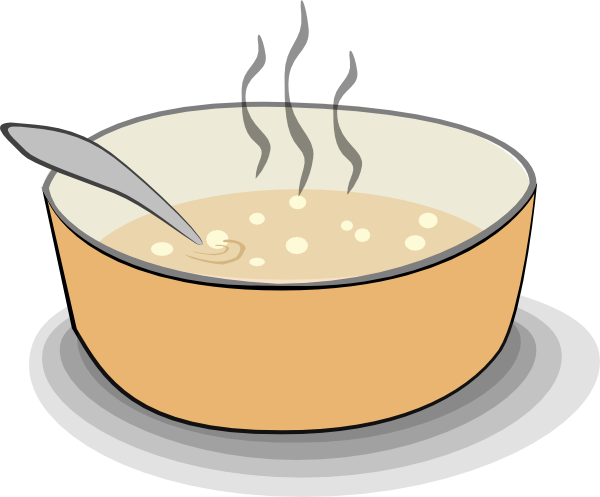
\includegraphics[width=0.3\textwidth]{figures/soup}
\end{center}

\begin{itemize}

\item When you taste a spoonful of soup and decide the spoonful you tasted isn't salty 
enough, that's \hl{exploratory analysis}

\item If you generalize and conclude that your entire soup needs salt, that's an \hl{
inference}

\item For your inference to be valid, the spoonful you tasted (the sample) needs to be 
\hl{representative} of the entire pot (the population)

\end{itemize}

%---Note---%
\note{

tasting food analogy
\begin{itemize}
\item do you taste entire pot to see if it is salty enough.

\item one taste: exploratory analysis.

\item going from taste, to entire pot is inference.  this soup is too salty.

\item if you haven't mixed things up are you actually going to get a representative
smaple.

\item you need to mix things up to get representative sample.
\end{itemize}

}

\end{frame}

%%%%%%%%%%%%%%%%%%%%%%%%%%%%%%%%%%%

\subsection{Ideally use a simple random sample, stratify to control for a variable, and cluster to make sampling easier} 
\label{mi2}

%%%%%%%%%%%%%%%%%%%%%%%%%%%%%%%%%%%

\begin{frame}
\frametitle{2. Ideally use a simple random sample, stratify to control for a variable, 
and cluster to make sampling easier}

\pause

\twocol{0.505}{0.51}{
\hl{Simple random:} \\
{\small Drawing names from a hat}
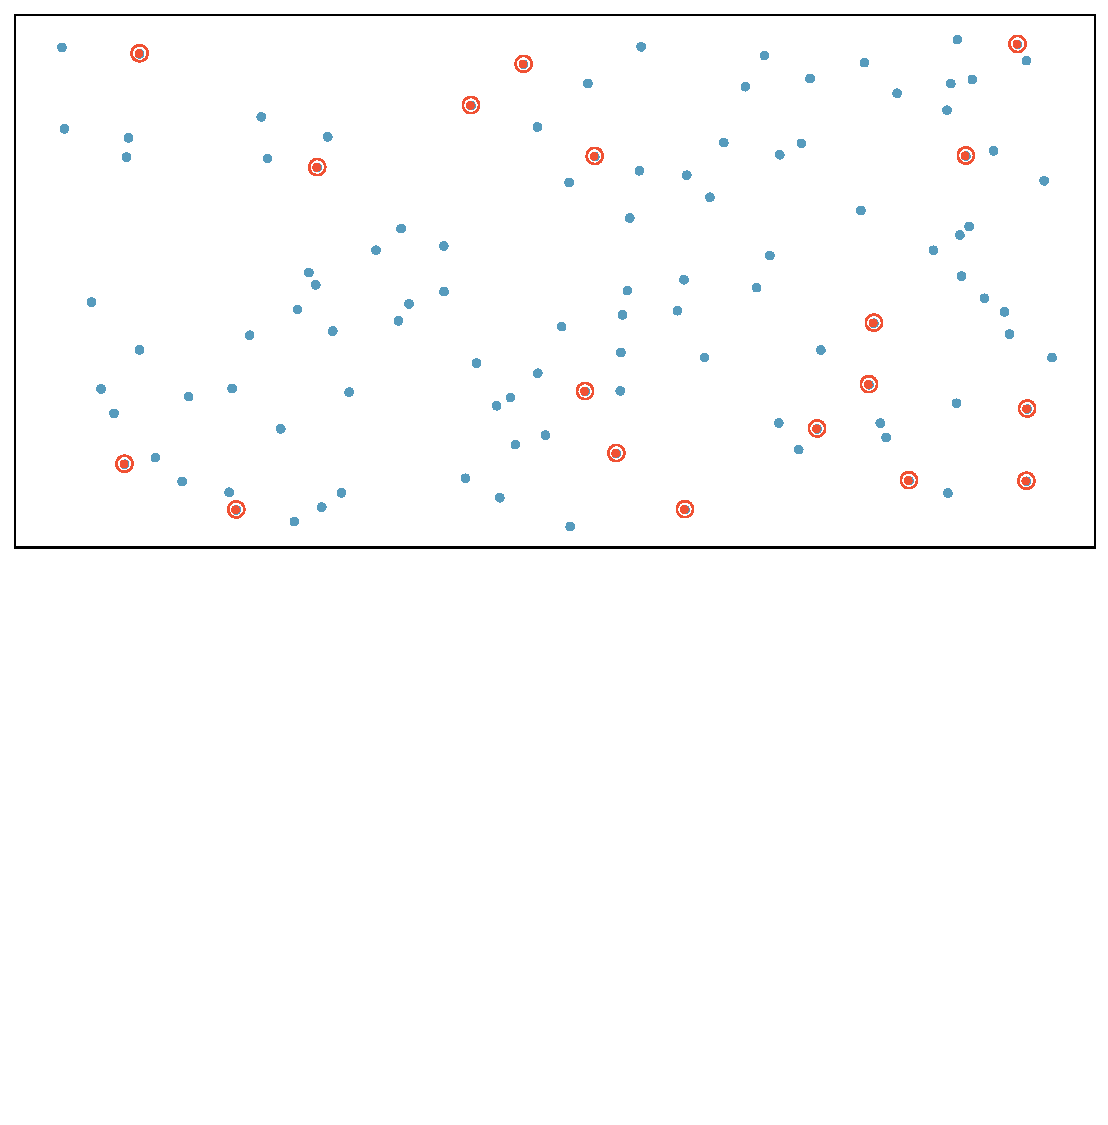
\includegraphics[width=\textwidth]{figures/sampling_simple} \\
\pause
\hl{Stratified:} {\small homogenous strata} \\
{\small Stratify to control for SES} \\
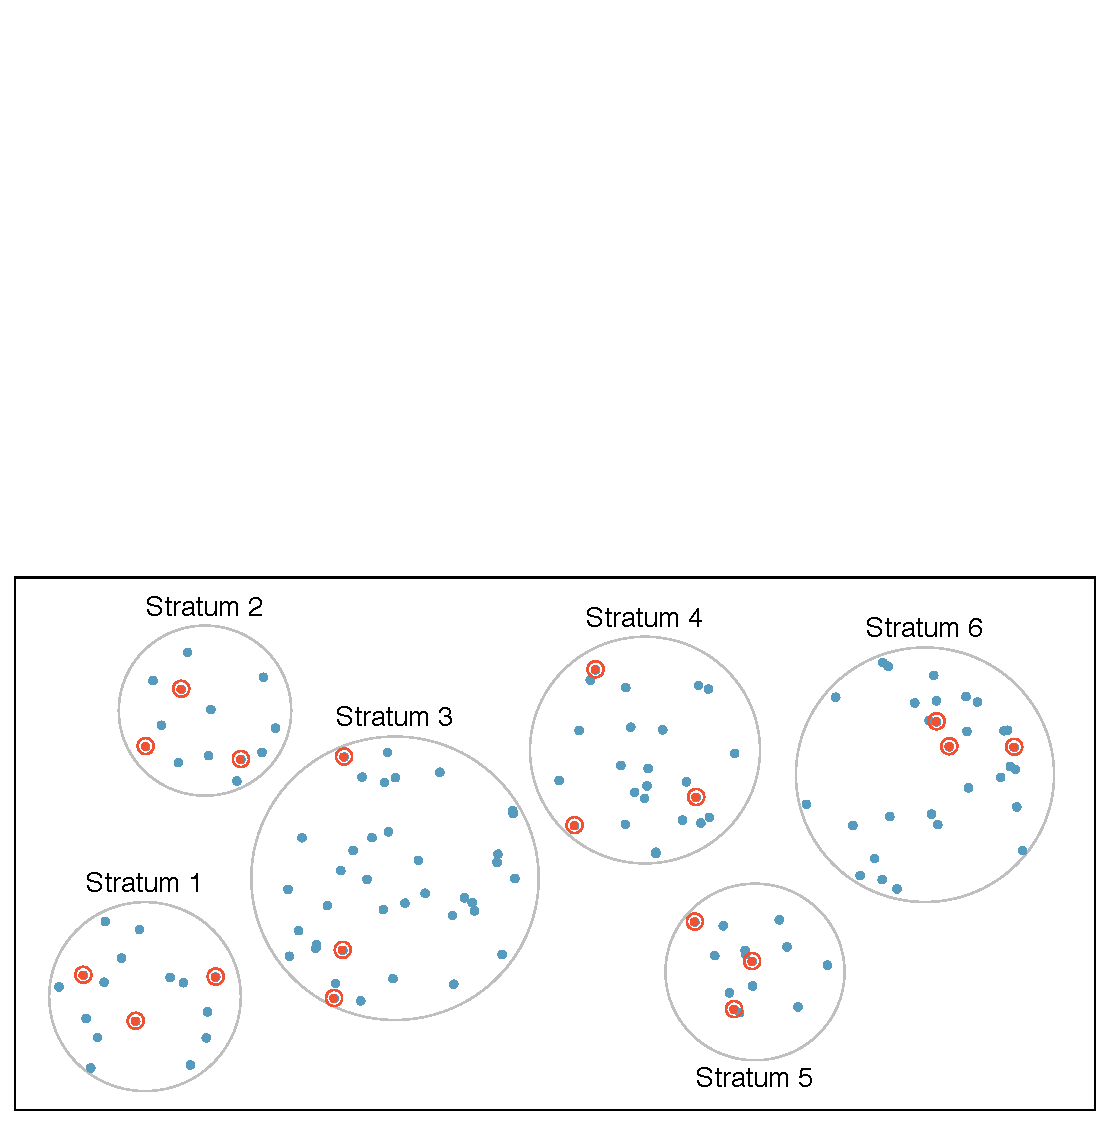
\includegraphics[width=\textwidth]{figures/sampling_stratified} 
}
{
\pause
\hl{Cluster:} {\small heterogenous clusters} \\
{\small Sample all chosen clusters}
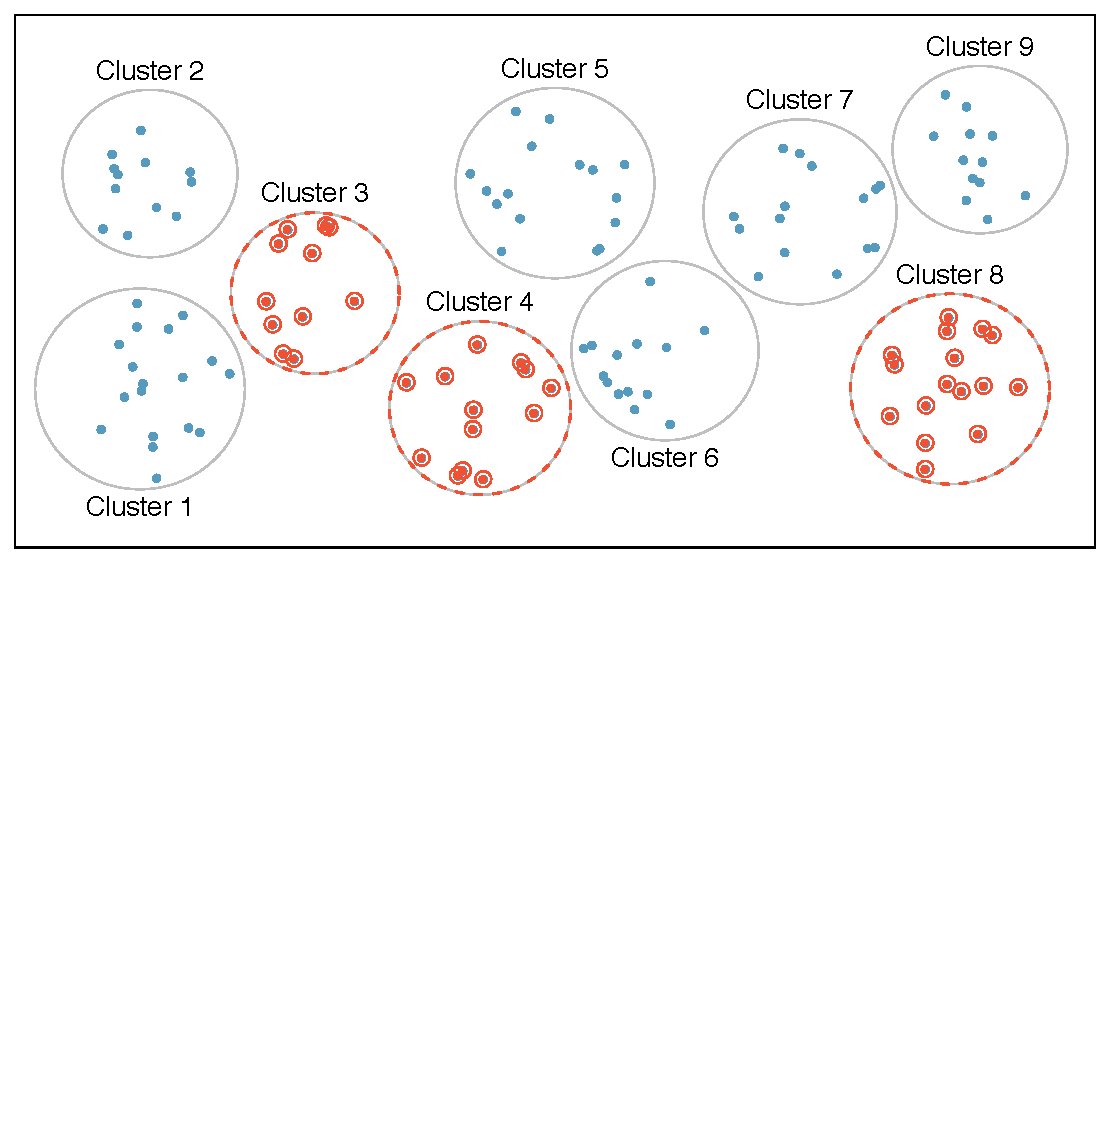
\includegraphics[width=\textwidth]{figures/sampling_cluster} \\
\pause
\hl{Multistage:} \\
{\small Random sample in chosen clusters}
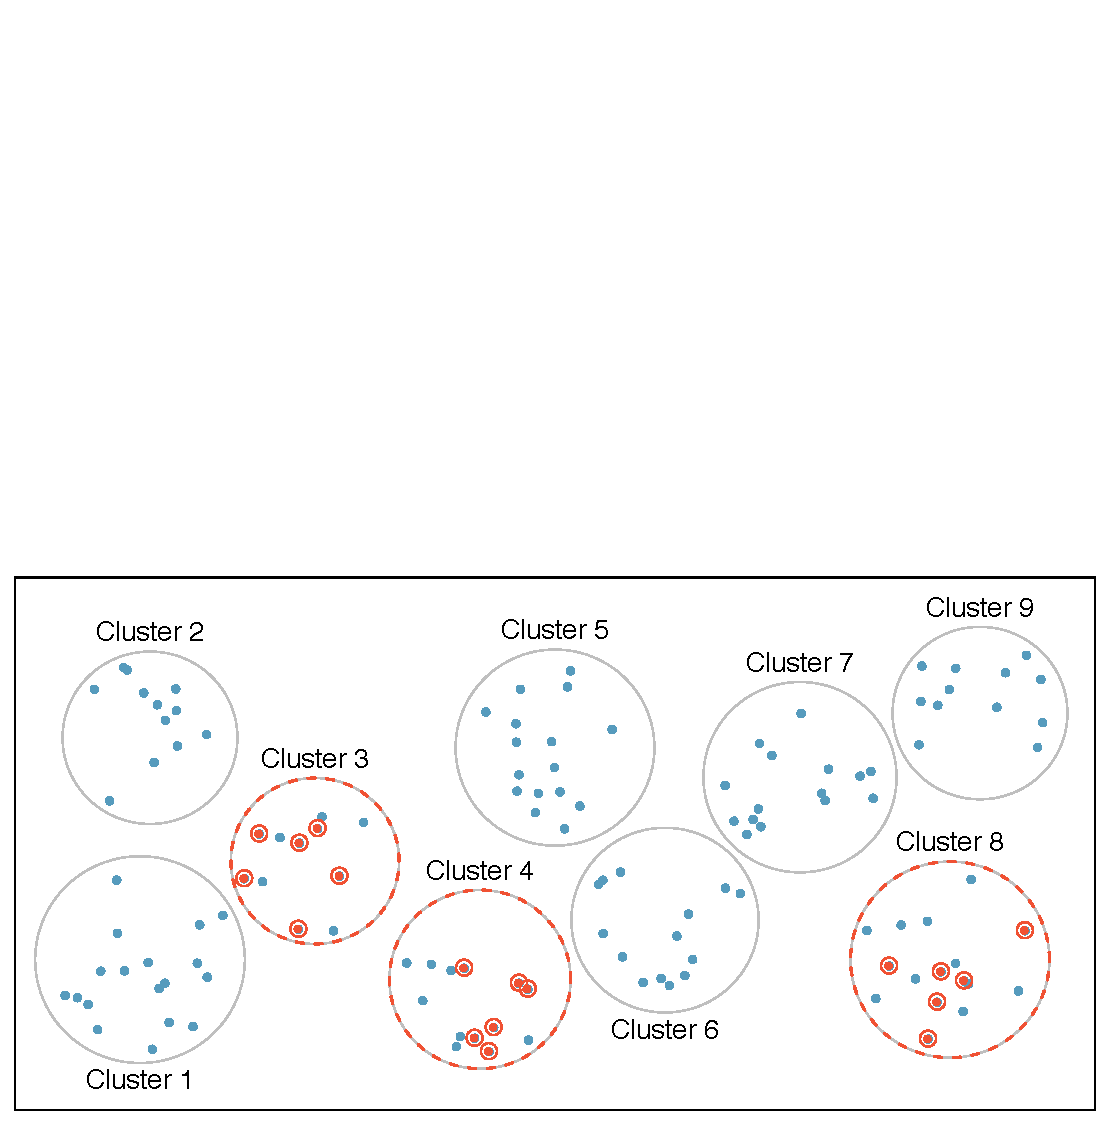
\includegraphics[width=\textwidth]{figures/sampling_multistage}
}

%---Note---%
\note{

Simple random sampling:
\begin{itemize}
\item simple random sample is equally likely to be selected.
\end{itemize}

Stratified sampling:
\begin{itemize}
\item when stratifying, first group by what is common about them, say socio-economic status.  Then go into each group, each strata, and randomly sample.
\end{itemize}

Clustering:
\begin{itemize}
\item maybe based on geographical information or something like that.
\item figure out what clusters are, since you don't have resources, pick just some clusters, and then sample.
\item ideally, clusters are similar
\item if clusters are similar then this isn't going to be a problem.
\end{itemize}

R: when might you use clustering?
\begin{itemize}
\item schools very similar in school district.
\item first sample a few schools.  then send surveys.
\end{itemize}

Lots of us surveys do clustering by county
}

\end{frame}

%%%%%%%%%%%%%%%%%%%%%%%%%%%%%%%%%%%

\begin{frame}

\clicker{A city council has requested a household survey be conducted in a suburban 
area of their city. The area is broken into many distinct and unique neighborhoods, 
some including large homes, some with only apartments, and others a diverse mixture of 
housing structures. Which approach would likely be the \emph{least} effective?}

\begin{enumerate}[(a)]
\item Simple random sampling
\item Stratified sampling, where each stratum is a neighborhood
\item \solnMult{Cluster sampling, where each cluster is a neighborhood}
\end{enumerate}

%---Note---%
\note{

Clicker question: read question and answers, 45-50 seconds.

C is most popular by far.  Someone that chose C, why?  clusters sound dissimilar.

Give exmaple of duke forrest, lots of Professors live there. That isn't representative of Durhams population.

}

\end{frame}

%%%%%%%%%%%%%%%%%%%%%%%%%%%%%%%%%%%

\subsection{Sampling schemes can suffer from a variety of biases}
\label{mi3}

%%%%%%%%%%%%%%%%%%%%%%%%%%%%%%%%%%%

\begin{frame}
\frametitle{3. Sampling schemes can suffer from a variety of biases}

\begin{itemize}[<+->]

\item \hl{Non-response:} If only a small fraction of the randomly sampled people choose 
to respond to a survey, the sample may no longer be representative of the population

\item \hl{Voluntary response:} Occurs when the sample consists of people who volunteer 
to respond because they have strong opinions on the issue since such a sample will also 
not be representative of the population

\item \hl{Convenience sample:} Individuals who are easily accessible are more likely to 
be included in the sample

\end{itemize}

%---Note---%
\note{

Non-response: 
\begin{itemize}
\item R: when do we generally have non-response errors?
\item when we have reached out to sample and people still refuse to respond.
\end{itemize}

Voluntary response bias:
\begin{itemize}

\item voluntary response issue: people volunteer to respond.  

\item cnn always has a poll.  disclaimer: this is not a scientific poll.

\item Q: who takes time to repsond to somethign that shows up on screen?

\item people that have really strong opinions.

\end{itemize}

The big distinction between voluntary and non-response is that with non-response the 
person designing the survey has done everything possible to avoid biasing the results.  
Voluntary response may be due to a lack of effort on the part of the scientist.

convenience samples:
\begin{itemize}

\item individuals who are easily accessible are more likely to be included

\item ask friends, friends more likely to be like minded

\item how much you work out, and you like to work out, and you run survey at gym...

\end{itemize}

}

\end{frame}

%%%%%%%%%%%%%%%%%%%%%%%%%%%%%%%%%%%

\begin{frame}[shrink]

{\small
\clicker{A school district is considering whether it will no longer allow high school 
students to park at school after two recent accidents where students were severely 
injured. As a first step, they survey parents by mail, asking them whether or not the 
parents would object to this policy change. Of 6,000 surveys that go out, 1,200 are 
returned. Of these 1,200 surveys that were completed, 960 agreed with the policy change 
and 240 disagreed. Which of the following statements are true?}

\begin{enumerate}[I.]
\item Some of the mailings may have never reached the parents.
\item Overall, the school district has strong support from parents to move forward with 
the policy approval.
\item It is possible that majority of the parents of high school students disagree with 
the policy change.
\item The survey results are unlikely to be biased because all parents were mailed a 
survey. 
\end{enumerate}

\begin{multicols}{5}
\begin{enumerate}[(a)]
\item Only I
\item I and II
\item \solnMult{I and III}
\item III and IV
\item Only IV
\end{enumerate}
\end{multicols}
}

\end{frame}

%%%%%%%%%%%%%%%%%%%%%%%%%%%%%%%%%%%%

\subsection{Experiments use random assignment to treatment groups, observational studies do not}
\label{mi4}

%%%%%%%%%%%%%%%%%%%%%%%%%%%%%%%%%%%%

\begin{frame}
\frametitle{}

\disc{What type of study is this? What is the scope of inference (causality / generalizability)?}

\begin{center}
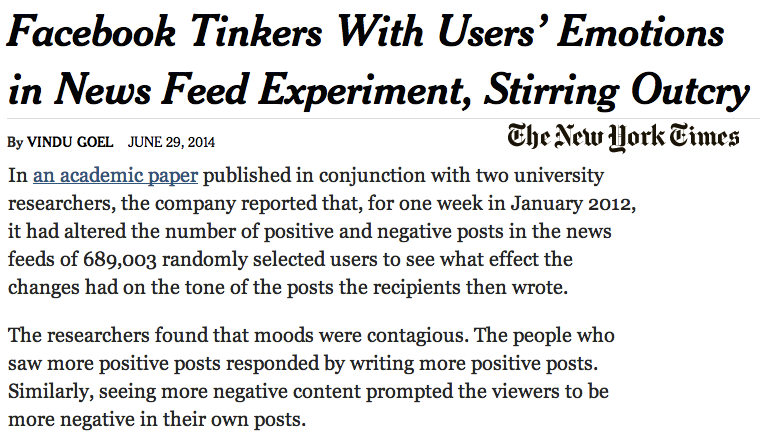
\includegraphics[width=0.9\textwidth]{figures/facebook_study}
\end{center}

\ct{\webURL{http://www.nytimes.com/2014/06/30/technology/facebook-tinkers-with-users-emotions-in-news-feed-experiment-stirring-outcry.html}}

%---Note---%
\note{

Facebook example:
\begin{itemize}
\item go over difference between experiements and observational studies.  Random assignment.  Random sampling.

\item News with facebook, they published a paper in conjuction with researchers... read from article.

\item Q: what type of study is this? experment.

\item Q: why?  they were actually randomly assigning people.

\item R: how would we make this an observational study?

\item What is the scope of inference.  Q: What can we say about causality, what can we talk about generalizability?

\item R: what does causality require: random assignment

\item R: what does generalizabiltiy require: random sample.

\item Facebook got in big trouble: didn't tell anybody.  big no-no in research.

\end{itemize}

}

\end{frame}

%%%%%%%%%%%%%%%%%%%%%%%%%%%%%%%%%%%%%

\begin{frame}
\frametitle{4. Experiments use random assignment to treatment groups, observational studies do not}

{\small
\disc{A study that surveyed a random sample of otherwise healthy adults found that people are more likely to get muscle cramps when they're stressed. The study also noted that people drink more coffee and sleep less when they're stressed. What type of study is this?}

\soln{\onslide<2->{Observational}}

\disc{What is the conclusion of the study?}

\soln{\onslide<3->{There is an \hl{association} between increased stress \& muscle cramps.}}

\disc{Can this study be used to conclude a causal relationship between increased stress and muscle cramps?}

\soln{\onslide<4->{Muscle cramps might also be due to increased caffeine consumption or sleeping less -- these are potential \hl{confounding} variables.}}
}

%---Note---%
\note{

Muscle cramp study:
\begin{itemize}
\item Read about study.

\item Q: What type of study? observational.

\item What is the conclusion, what type of wording would be appropriate?  There is an association between these things.

\item Can we make a causal statement?  no.

\item Read.  we don't know if it is whatever or whatever.  what we call these are potential confounding variables.
\end{itemize}

}

\end{frame}

%%%%%%%%%%%%%%%%%%%%%%%%%%%%%%%%%%%%

\subsection{Four principles of experimental design: randomize, control, block, replicate}
\label{mi5}

%%%%%%%%%%%%%%%%%%%%%%%%%%%%%%%%%%%%

\begin{frame}
\frametitle{5. Four principles of experimental design:\\ randomize, control, block, 
replicate}

\begin{itemize}
\item We would like to design an experiment to investigate if increased stress causes 
muscle cramps:

\pause

\begin{itemize}
\item Treatment: increased stress
\item Control: no or baseline stress
\end{itemize}

\pause

\item It is suspected that the effect of stress might be different on younger and older 
people: \hl{block} for age.

\end{itemize}

\pause

\disc{Why is this important? Can you think of other variables to block for?}

%---Note---%
\note{

Four principles of experimental design.

\begin{itemize}
\item We want to know if increased stress CAUSES muscle cramps.  Need random assignment.
\item Effect of stress might be different on younger than older people.  Block for age if you think age will effect how people will respond.  Then do random assignment within each group.
\item Q: What other variables might we block for?  Sex/gender.  You want the same number of males and females in each group.
\item Blocking gives us an equal distribution of each group to the control and experiment.
\end{itemize}

}

\end{frame}

%%%%%%%%%%%%%%%%%%%%%%%%%%%%%%%%%%%

\subsection{Random sampling helps generalizability, random assignment helps causality}
\label{mi6}

%%%%%%%%%%%%%%%%%%%%%%%%%%%%%%%%%%%%

\begin{frame}
\frametitle{6. Random sampling helps generalizability,\\ random assignment helps 
causality}

\begin{center}
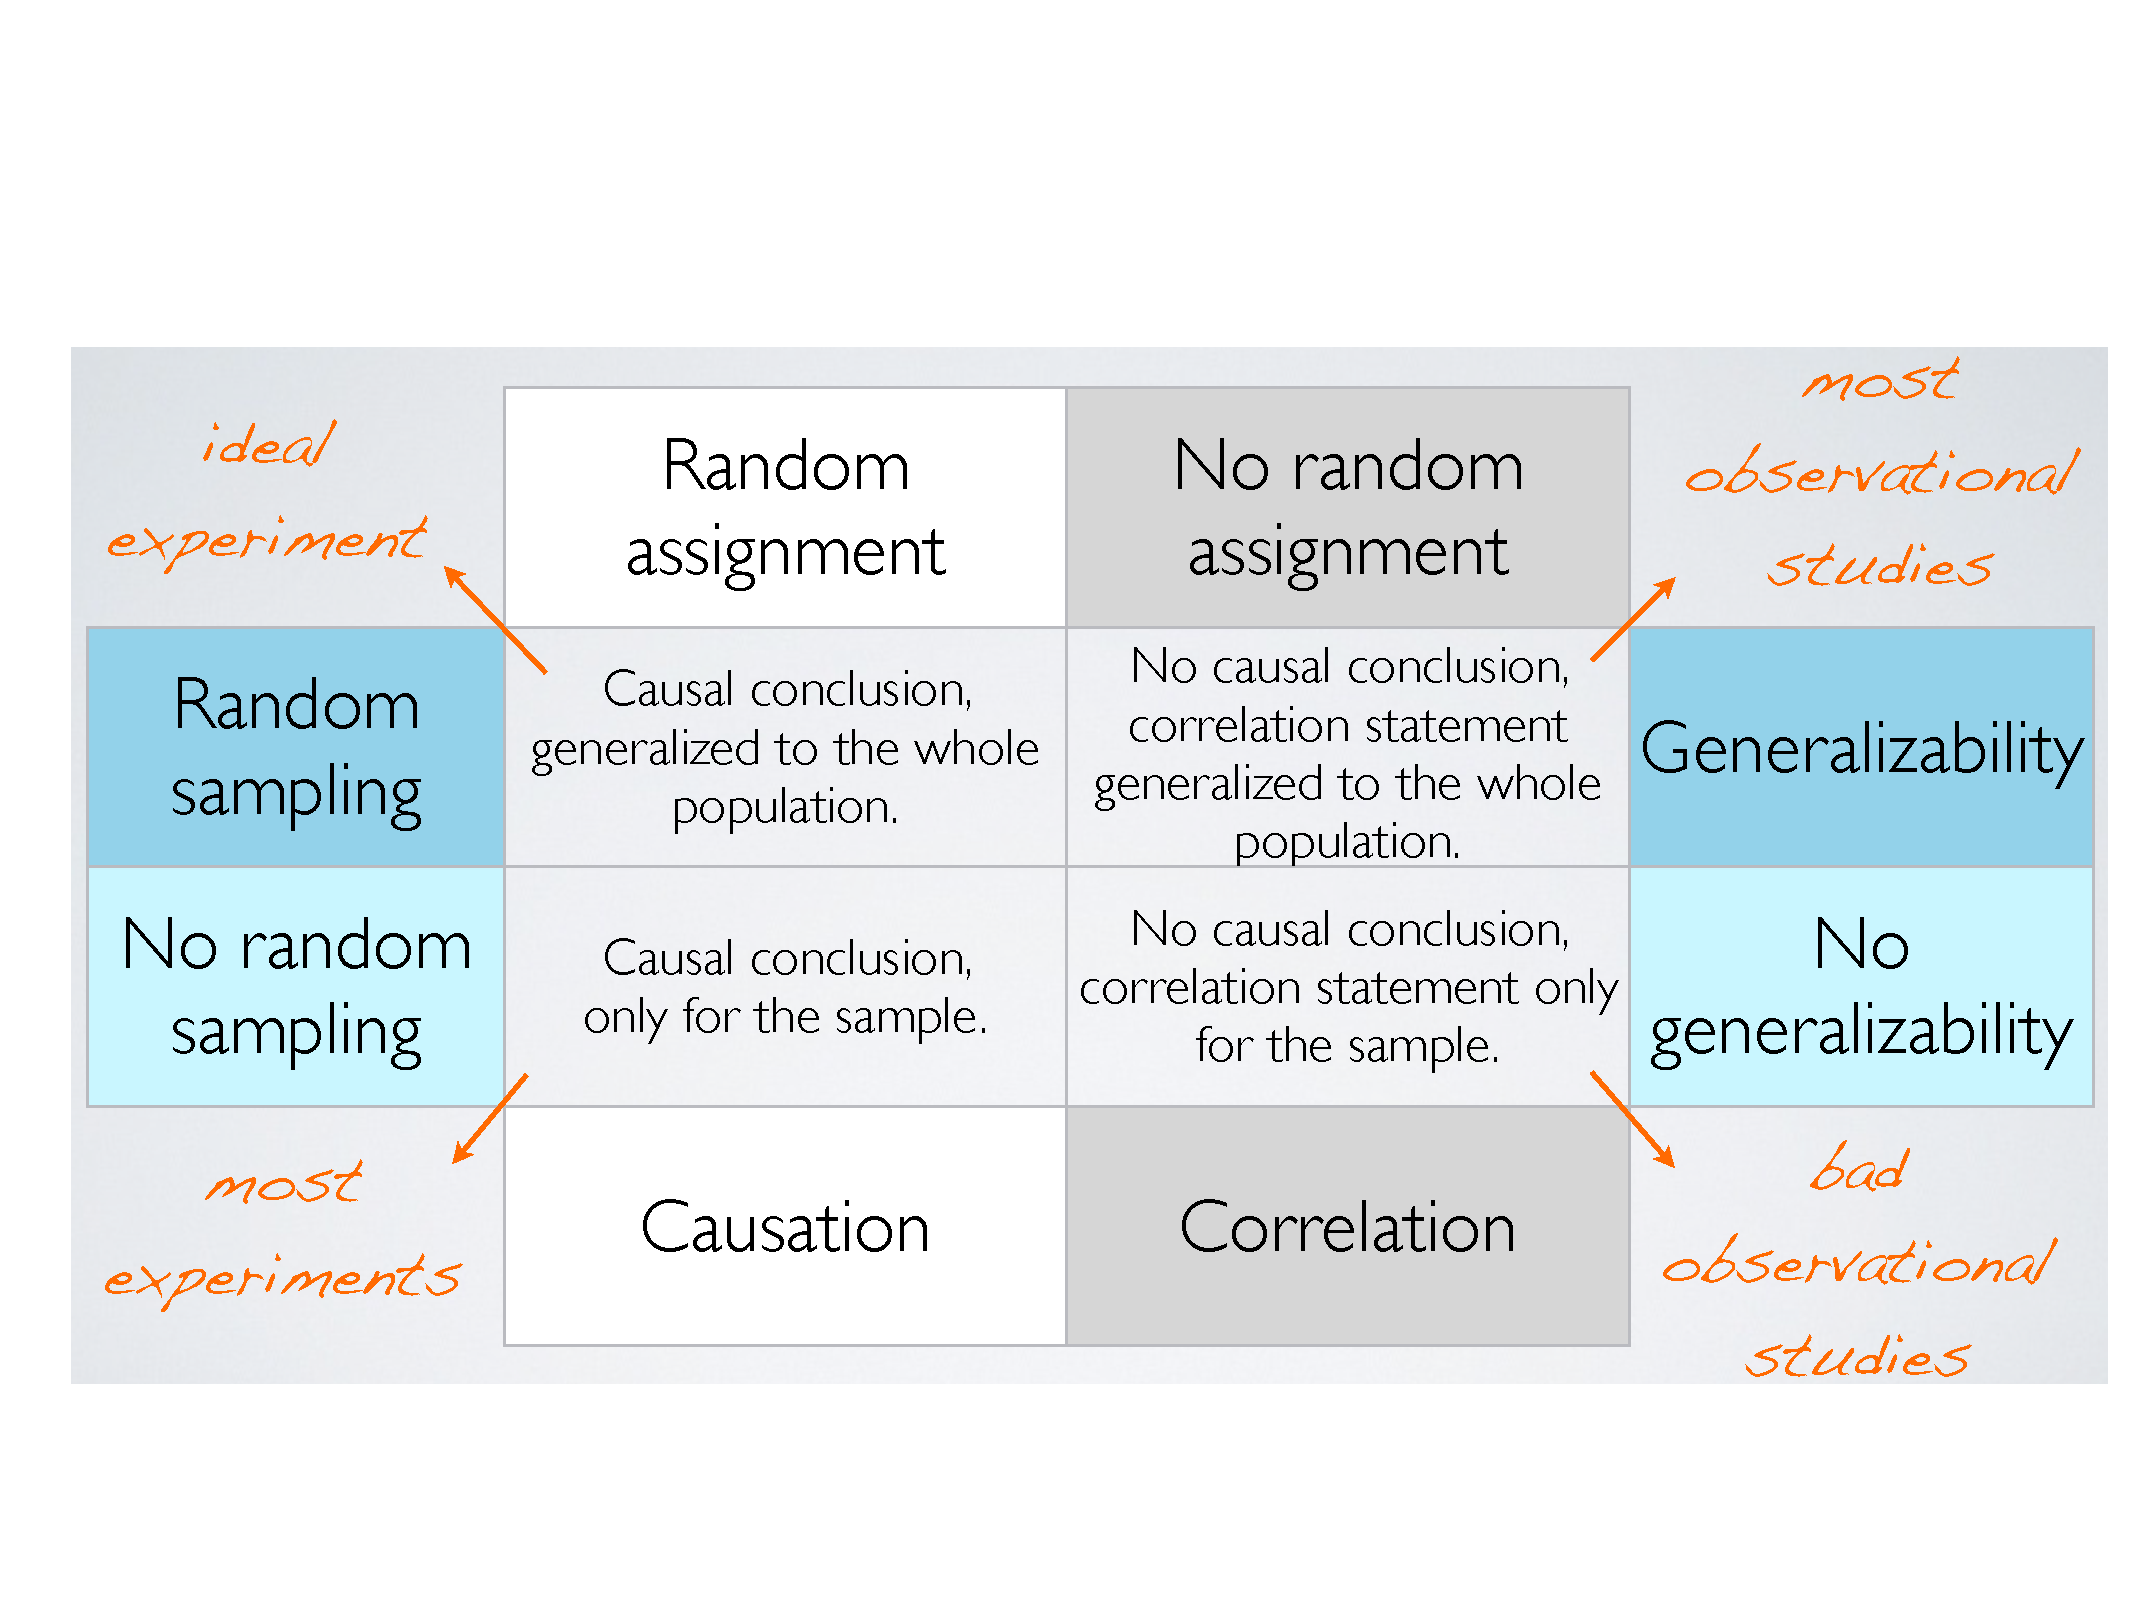
\includegraphics[width=\textwidth]{figures/random_sample_assignment}
\end{center}

%---Note---%
\note{

random assignment: causality

random sample is hard to get: rarely we will get these.

volunteers: voluntary response bias.

usually most experiments lower left.

most surveys: upper right. (social sciences)

lower right: weakest type of study.

}

\end{frame}

%%%%%%%%%%%%%%%%%%%%%%%%%%%%%%%%%%%

\section{Class survey [time permitting]}

%%%%%%%%%%%%%%%%%%%%%%%%%%%%%%%%%%%%

\begin{frame}
\frametitle{}

\activity{Class survey}
{
\begin{itemize}
    \setlength{\itemsep}{0pt}
    \setlength{\parskip}{0pt}
\item One of your first tasks in this class is to help design a survey. This survey 
will be completed \emph{anonymously}. It will (ideally) have information on \emph{
variables you are interested in}. When writing your question consider whether you 
would feel comfortable answering it on an anonymous survey.

\item Work with 3-4 classmates to come up with a survey question, and add it to Google 
Doc linked below. Make sure that the wording of the question is clear, and (if 
categorical) the answer choices make sense.
\begin{center}
\webURL{http://bit.ly/sta101f15_ClassSurvey}
\end{center}

\item Before adding a question check to make sure that it hasn't already been added. 
If your question is already there, but you can suggest a clearer / better wording, add 
it as ``alternative wording'' underneath the original question.
\end{itemize}
}

%---Note---%
\note{

  \begin{itemize}
    \item Work in informal teams of 3-4.
    \item Go over examples of types of questions.
    \item Come up with questions.
    \item Do not put questions you (or another) would be uncomfortable answering.
    \item But try to keep the questions interesting.
    \item We will try to compile a set of reasonable questions for you all to answer.
    \item You will fill out the survey and then we will use that data for examples during the semester.
  \end{itemize}

}

\end{frame}

%%%%%%%%%%%%%%%%%%%%%%%%%%%%%%%%%%%%

\section{Summary}

%%%%%%%%%%%%%%%%%%%%%%%%%%%%%%%%%%%

\begin{frame}
\frametitle{Summary of main ideas}

\vfill

\begin{enumerate}

\item \nameref{mi1}

\item \nameref{mi2}

\item \nameref{mi3}

\item \nameref{mi4}

\item \nameref{mi5}

\item \nameref{mi6}

\end{enumerate}

\vfill

\end{frame}

%%%%%%%%%%%%%%%%%%%%%%%%%%%%%%%%%%%

\end{document}